\section{Zufallsvariablen}


\begin{LA}
    {}{IntroZV-EW}
    Alice spielt das Glücksspiel `Chuck-a-Luck'

    Dabei handelt es sich um ein einfaches Glücksspiel mit drei Würfeln. Die Spieler tätigen ihre Einsätze auf einem Tableau mit den Zahlen Eins bis Sechs, anschliessend wirft der Bankhalter, d.h. der Spielleiter, drei Würfel.

    Zeigt ein Würfel die gesetzte Augenzahl, gewinnt der Spieler einfach, d.h. er erhält seinen Einsatz zurück und bekommt noch einmal die gleiche Summe. Für jeden weiteren Würfel, der die gesetzte Augenzahl anzeigt, erhält er nochmals die eingesetzte Summe. Zeigt kein Würfel die gesetzte Augenzahl, so ist der Einsatz verloren.

    \begin{enumerate}
    \item Berechne die Wahrscheinlichkeit, dass beim Setzen auf «Sechs» und einem Einsatz von einem Franken ein Gewinn von drei Franken, zwei Franken, einem Franken, von minus einem Franken (d.h. ein Verlust) erzielt wird.

    \item Führe das Spiel zehnmal durch. Wie hoch ist dabei der durchschnittliche Gewinn pro Spiel?

    \item Wie hoch vermutest du den durchschnittlichen Gewinn/Verlust des Spielers pro Spiel auf lange Sicht, d.h. wenn beliebig oft gespielt wird?

    \item Ein Spiel heisst fair, wenn der durchschnittliche Gewinn auf lange Sicht null ist. Ist Chuck-a-Luck ein faires Spiel?
    \end{enumerate}

\end{LA}

\clearpage
\subsection{Zufallsvariable und Verteilung}
Wir haben bisher bereits einige Fragen der folgenden Art untersucht:

\begin{itemize}
\item Mit welcher Wahrscheinlichkeit ist die Augensumme beim Wurf von zwei Würfeln 4?
\item Mit welcher Wahrscheinlichkeit fällt eine Münze bei fünfmaligem Werfen genau einmal auf Kopf?
\item Aus einer Urne mit 6 schwarzen und 3 weissen Kugeln werden drei Kugeln gezogen. Mit welcher Wahrscheinlichkeit sind genau zwei davon schwarz?
\end{itemize}

Alle diese Ereignisse umfassen mehrere Ergebnisse. Bei den Würfeln wären das z.\,B. die Ergebnisse \((1,3)\), \((3,1)\) und \((2,2)\) und bei der Münze KZZZZ, ZKZZZ, usw. Diese Ergebnisse werden zusammengefasst, weil sie eine gemeinsame Eigenschaft haben. Im ersten Fall ist die Gemeinsamkeit die Augensumme, im zweiten die Anzahl Münzen, die auf Kopf fallen.


Die Grösse, die untersucht wird, nennt man \textbf{Zufallsvariable} oder \textbf{Zufallsgrösse}.
Sie wird häufig mit \( X \) bezeichnet.
In den genannten Beispielen wird als Zufallsvariable einmal die Augensumme von zwei Würfeln, einmal die Anzahl Köpfe und einmal die Anzahl schwarzen Kugeln betrachtet.

\begin{definition}
    {Zufallsvariable}{}
    Eine \textit{Zufallsvariable} (auch Zufallsgrösse) \( X \) ordnet jedem Ergebnis \( s_i \) eines Zufallsversuchs eine Zahl zu.

    Die möglichen Werte von \( X \) werden mit \( x_1,\, x_2,\, x_3,\, \ldots,\, x_n \) bezeichnet.

    \medskip

    Das Ereignis, das aus allen Ergebnissen des Zufallsversuchs besteht, für welche die Zufallsgrösse \( X \) den Wert \( x_k \) annimmt, wird mit \( X = x_k \) bezeichnet.

    
    \(
    P(X = x_k) = p_k
    \)
    bezeichnet die Wahrscheinlichkeit, dass die Zufallsgrösse \( X \) den Wert \( x_k \) annimmt.

\end{definition}

\medskip

Die \textbf{Verteilung} einer Zufallsgrösse ist die Zuordnung, welche jedem möglichen Wert der Zufallsvariable die entsprechende Wahrscheinlichkeit zuordnet.

\begin{bsp}
    {Chuck-a-Luck}{}
    Die Zufallsvariable, die in \cref{LA:IntroZV-EW} untersucht wurde, ist $X:$ `Gewinn in einer Partie Chuck-a-Luck'.

    Die möglichen Werte der Zufallsvariable sind $x_1 = -1, x_2 = 1, x_3 = 2, x_4 =3$. 

    Die Wahrscheinlichkeit, dass man bei Chuck-a-Luck den Gewinn 3 erzielt, wird so notiert:

    $$p_4 = P(X=3) = \left(\frac{1}{6}\right)^3$$

    Die möglichen Werte und zugehörigen Wahrscheinlichkeiten kann man in einer Tabelle erfassen:

    \begin{center}
    \begin{tabular}{|c|c|c|c|c|c|}
    \hline
    $x_k$ & $-1$ & $1$ & $2$ & $3$& $\Sigma$\\ \hline
    $p_k$ & $125/216$ & 75 /216 & 15/216 & 1/216 & $216/216 = 1$ \checkmark
  \\ \hline
    %$p_k$ & $0.5787$ & $0.3472$ & $0.0694$ & $0.0046$ \\ \hline
    % $p_k$ & $\left(\frac{5}{6}\right)^3$ & $3 \cdot \frac{1}{6} \cdot \left(\frac{5}{6}\right)^2$ & $3 \cdot \left(\frac{1}{6}\right)^2 \cdot \frac{5}{6}$ & $\left(\frac{1}{6}\right)^3$ 
    \end{tabular}
  \end{center}
Die Summe der einzelnen Wahrscheinlichkeiten müssen 1 bzw. 100\% ergeben. Das ist eine gute Möglichkeit, die Wahrscheinlichkeiten zu kontrollieren\dots

Die Wahrscheinlichkeiten werden häufig auch mit einem Stabdiagramm visualisiert:
  
\begin{center}
    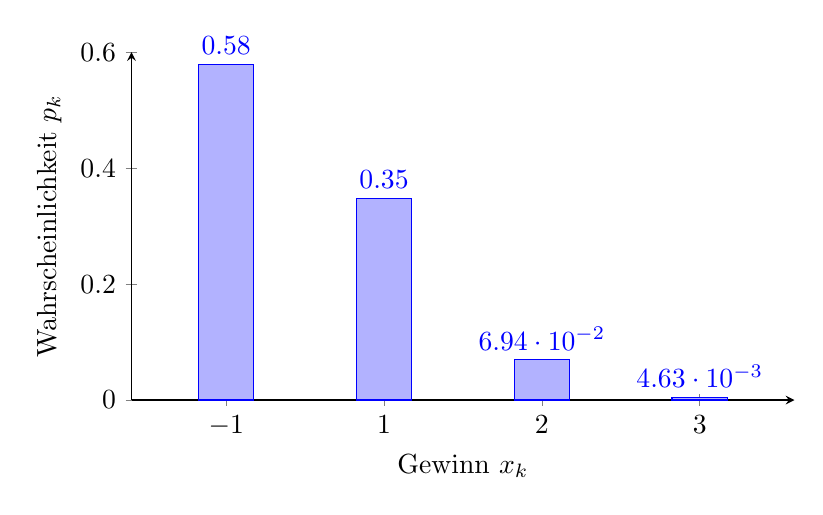
\begin{tikzpicture}
\begin{axis}[
    ybar,
    ymin=0,
    ymax=0.6,
    ylabel={Wahrscheinlichkeit $p_k$},
    xlabel={Gewinn $x_k$},
    xtick=data,
    axis x line=bottom,
    axis y line=left,
    xticklabels={$-1$, $1$, $2$, $3$},
    bar width=20pt,
    width=10cm,
    height=6cm,
    nodes near coords,
    enlarge x limits=0.2
]
\addplot coordinates {
    (0, {(5/6)^3})
    (1, {3*(1/6)*(5/6)^2})
    (2, {3*(1/6)^2*(5/6)})
    (3, {(1/6)^3})
};
% \addplot coordinates {
%     (0, 0.5787)
%     (1, 0.3472)
%     (2, 0.0694)
%     (3, 0.0046)
% };
\end{axis}
\end{tikzpicture}
  \end{center}

\end{bsp}

\begin{definition}
    {Verteilung einer Zufallsvariable}{}
Für eine Zufallsgrösse \( X \) wird die Art, wie die 100\% auf die Wahrscheinlichkeiten \( p_1,\, p_2,\, \ldots,\, p_n \) der Werte \( x_1,\, x_2,\, \ldots,\, x_n \) aufgeteilt werden, die zur Zufallsgrösse \( X \) gehörende \textit{Verteilung} genannt. 
Die Verteilung einer Zufallsgrösse kann mit einem \textit{Stabdiagramm} visualisiert werden.

\end{definition}

\subsection{Erwartungswert}

\begin{bsp}
    {Einführungsbeispiel}{}
    Bei einem Glücksspiel wie Chuck-a-Luck stelt sich die Frage, ob sich die Teilnahme für den Spieler lohnt. Eine Grösse, die man dafür untersuchen kann ist der sogenannte \emph{Erwartungswert}. Er gibt an, wie hoch der durchschnittliche Gewinn pro Spielrunde ist, wenn man das Spiel häufig durchführt.

    Um den Erwartungswert des Gewinns in Chuck-a-Luck zu berechnen, stellen wir uns vor, dass wir das Spiel 216-mal spielen. 
    
    


    \vspace*{5cm}


% Bei 216 Spielen ca. \\
% 125 $\times$ $-1$, \quad 75 $\times$ $1$, \quad 15 $\times$ $2$, \quad 1 $\times$ $3$

% \medskip

% \textbf{Durchschnittlicher Gewinn pro Spiel:}
% \[
% \frac{125 \cdot (-1) + 75 \cdot 1 + 15 \cdot 2 + 1 \cdot 3}{216}
% = (-1) \cdot \frac{125}{216} + 1 \cdot \frac{75}{216} + 2 \cdot \frac{15}{216} + 3 \cdot \frac{1}{216}
% = -\frac{17}{216}
% \]




\end{bsp}

\begin{definition}
    {Erwartungswert}{}
    Der \textit{Erwartungswert} \( E(X) \) einer Zufallsvariable \( X \) ist definiert als

    \[
    E(X) = x_1 \cdot p_1 + x_2 \cdot p_2 + x_3 \cdot p_3 + \ldots + x_{n-1} \cdot p_{n-1} + x_n \cdot p_n 
    = \sum_{k=1}^{n} x_k \cdot p_k
    \]

    Dabei entsprechen \( p_1,\, p_2,\, \ldots,\, p_{n-1},\, p_n \) den Wahrscheinlichkeiten, mit denen die Zufallsgrösse \( X \) ihre möglichen Werte \( x_1,\, x_2,\, \ldots,\, x_{n-1} \) und \( x_n \) annimmt.

\end{definition}

Der Erwartungswert kann effizient berechnet werden, wenn man die Tabelle für die Verteilung einer Zufallsvariable um eine Zeile erweitert:

\renewcommand{\arraystretch}{2} % Für die Höhe der Spalten in der Tabelle
\begin{bsp}
    {}{}
    Eine Münze wird so lange geworfen, bis das erste Mal Zahl erscheint; höchstens aber viermal. Wie viele Würfe sind zu erwarten?

    $X$: Anzahl Würfe
    \begin{center}
        \begin{tabular}{{|>{\centering\arraybackslash}m{2cm}|>{\centering\arraybackslash}m{2cm}|>{\centering\arraybackslash}m{2cm}|>{\centering\arraybackslash}m{2cm}|>{\centering\arraybackslash}m{2cm}|>{\centering\arraybackslash}m{2cm}|}}
        \hline
        $x_k$ & $1$ & $2$ & $3$ & $4$& $\Sigma$\\ \hline
        $p_k$ &  &  &  &  & \\ \hline
        $x_k \cdot p_k$ &&&&&
    \\ \hline
        %$p_k$ & $0.5787$ & $0.3472$ & $0.0694$ & $0.0046$ \\ \hline
        % $p_k$ & $\left(\frac{5}{6}\right)^3$ & $3 \cdot \frac{1}{6} \cdot \left(\frac{5}{6}\right)^2$ & $3 \cdot \left(\frac{1}{6}\right)^2 \cdot \frac{5}{6}$ & $\left(\frac{1}{6}\right)^3$ 
        \end{tabular}
    \end{center}

        \vspace*{5cm}
\end{bsp}
\renewcommand{\arraystretch}{1} % Zurücksetzen der Höhe

\begin{definition}
    {Faires Spiel}{}
    Ein Glücksspiel heisst \textit{fair}, wenn der Erwartungswert des Gewinns null ist, d.\,h. wenn auf lange Sicht keiner der Spieler (oder die Bank) einen Gewinn erwarten kann.
\end{definition}

\clearpage

%\section{TODO: Spannendere Aufgaben!}


\begin{ueb}
    {}{}
    \begin{enumerate}
\item Berechne den Erwartungswert der folgenden Verteilungen.
\begin{enumerate}
    \item 
    \[
    \begin{array}{c|ccccc}
    x_k & -5 & -4 & 1 & 3 & 6 \\ \hline
    p_k & 0.3 & p & 0.1 & 0.2 & 0.3
    \end{array}
    \]
    \item 
    \[
    \begin{array}{c|ccc}
    x_k & 3 & 7 & 8 \\ \hline
    p_k & \frac{1}{4} & \frac{1}{3} & p
    \end{array}
    \]
\end{enumerate}

\item Zwei Laplace-Würfel werden einmal geworfen. Die Zufallsgrösse \( X \) sei das Maximum der beiden Augenzahlen (bei (5/3) also 5, bei (4/4) 4, \ldots).
\begin{enumerate}
    \item Bestimme die Verteilung und den Erwartungswert von \( X \).
    \item Zeichne ein Säulendiagramm der Verteilung.
\end{enumerate}

% \item Eine Laplace-Münze wird geworfen, bis erstmals „Zahl“ oder viermal „Wappen“ erscheint.
% \begin{enumerate}
%     \item Mit wie vielen Würfen ist durchschnittlich zu rechnen?
%     \item Zeichne ein Säulendiagramm der Verteilung.
% \end{enumerate}

\item Einem Karton, der sechs ganze und zwei defekte Batterien enthält, werden zufällig vier Batterien entnommen. \\
Mit wie vielen defekten Batterien ist zu rechnen?


\item Alice schenkt Bob vier Salzige und drei gezuckerte Lebkuchenherze von gleicher Form. Bob isst ein Herz nach dem anderen, bis er erstmals in ein gezuckertes beisst. \\
Beim wievielten Herz ist dies durchschnittlich zu erwarten?

\item Alice und Bob beschliessen folgendes Spiel: Fünf Karten, auf denen die Zahlen 2, 3, 4, 5, 6 stehen, liegen verdeckt auf dem Tisch. Zwei Karten werden gezogen; ist die Summe der Zahlen gerade, gewinnt Alice 1 Fr., ist die Summe ungerade, gewinnt Bob 0.90 Fr. \\
Nach zwanzig Spielen hört einer der beiden frustriert auf. Warum?

\item Alice bezahlt Bob 7 Fr., wenn er in einem Wurf mit zwei Würfeln die Augensummen 5 oder 6 oder 7 wirft. In allen anderen Fällen gewinnt Alice den Einsatz von Bob. \\
Welchen Einsatz bezahlt Bob im Falle eines fairen Spiels?
\end{enumerate}

\end{ueb}

\clearpage
\emph{Lösungen:}
\begin{enumerate}
\item Erwartungswerte:
\begin{enumerate}
    \item $p= 0.1$, $E(X) =0.6$
    \item $p= 5/12$, $E(X) =77/12$
\end{enumerate}

\item Zwei Laplace-Würfel, Maximum:
\begin{enumerate}
    \item Erwartungswert $\approx 4.47$
    \item \dots
\end{enumerate}

% \item Laplace-Münze bis „Zahl“ oder viermal „Wappen“:
% \begin{enumerate}
%     \item Erwartungswert $= 1.9375$
%     \item \dots
% \end{enumerate}

\item Erwartete Anzahl defekter Batterien: $= 1$

\item Erwartete Position erster gezuckerter Brezel: $= 2$

\item Nachteil für Alice (sie verliert im Schnitt pro Spiel): Bob hat Vorteil $\approx 0.14$ Fr. pro Spiel

\item Fairer Einsatz für Bob: $\approx 5$ Fr.
\end{enumerate}























\clearpage
\subsection{Varianz und Standardabweichung}
\begin{LA}
    {Teil 1}{VarianzTeil1}
    Betrachten Sie die folgenden Wetten:
    
    \bigskip
    
    Wette 1: Ein Würfel wird einmal geworfen. Bei den Augenzahlen 1 oder 2, gewinnen Sie 9 CHF, andernfalls verlieren Sie 3 CHF.
    
    \bigskip
    
    Wette 2: Ein Würfel wird einmal geworfen. Bei den Augenzahlen 1 oder 2, gewinnen Sie 109 CHF, andernfalls verlieren Sie 53 CHF.

    \bigskip

    Seien $X$ und $Y$  die Zufallsvariablen $X$: \emph{Gewinn in CHF bei Wette 1} und $Y$: \emph{Gewinn in CHF bei Wette 2}. Füllen Sie die Tabellen unten und berechnen Sie die Erwartungswerte $E(X)$ und $E(Y)$.


\renewcommand{\arraystretch}{2} % Für die Höhe der Spalten in der Tabelle

      \begin{center}
        \begin{tabular}{{|>{\centering\arraybackslash}m{2cm}|>{\centering\arraybackslash}m{2cm}|>{\centering\arraybackslash}m{2cm}|>{\centering\arraybackslash}m{2cm}|}}
        \hline
        $x_k$ & $9$ & $-3$ & $\Sigma$\\ \hline
        $p_k$ &  &   & \\ \hline
        $x_k \cdot p_k$ &&&
    \\ \hline
        \end{tabular}
    \end{center}

    \bigskip

\begin{center}
        \begin{tabular}{{|>{\centering\arraybackslash}m{2cm}|>{\centering\arraybackslash}m{2cm}|>{\centering\arraybackslash}m{2cm}|>{\centering\arraybackslash}m{2cm}|}}
        \hline
        $y_k$ &  &  & $\Sigma$\\ \hline
        $p_k$ &  &   & \\ \hline
        $y_k \cdot p_k$ &&&
    \\ \hline
        \end{tabular}
    \end{center}

\renewcommand{\arraystretch}{1} % Für die Höhe der Spalten in der Tabelle


\end{LA}

\clearpage

\begin{LA}
    {Teil 2}{}
    Wir untersuchen die beiden Wetten aus \cref{LA:VarianzTeil1} genauer. Offenbar liegen die Werte der Zufallsvariable $X$ näher beim Erwartungswert als jene von $Y$.
    
    \bigskip
    
    Um diesen Unterschied zu messen, berechnen wir die erwartete Abweichung vom Erwartungswert. In anderen Worten: Wir betrachten die Zufallsvariablen $V = X - 1$ und $W = Y -1$.

\bigskip

Berechnen Sie die Erwartungswerte $E(V)$ und $E(W)$.
\renewcommand{\arraystretch}{2} % Für die Höhe der Spalten in der Tabelle
    \begin{center}
        \begin{tabular}{{|>{\centering\arraybackslash}m{2cm}|>{\centering\arraybackslash}m{2cm}|>{\centering\arraybackslash}m{2cm}|>{\centering\arraybackslash}m{2cm}|}}
        \hline
        $v_k$ & $8$ & $-4$ & $\Sigma$\\ \hline
        $p_k$ &  &   & \\ \hline
        $v_k \cdot p_k$ &&&
    \\ \hline
        \end{tabular}
    \end{center}

    \bigskip

\begin{center}
        \begin{tabular}{{|>{\centering\arraybackslash}m{2cm}|>{\centering\arraybackslash}m{2cm}|>{\centering\arraybackslash}m{2cm}|>{\centering\arraybackslash}m{2cm}|}}
        \hline
        $w_k$ &  &  & $\Sigma$\\ \hline
        $p_k$ &  &   & \\ \hline
        $w_k \cdot p_k$ &&&
    \\ \hline
        \end{tabular}
    \end{center}

\renewcommand{\arraystretch}{1} % Für die Höhe der Spalten in der Tabelle

\end{LA}

\clearpage

\begin{definition}
    {Varianz}{}
    Die Varianz $\operatorname{Var}(X)$ einer Zufallsvariable $X$ mit dem Erwartungswert $E(X) = \mu$ ist definiert als
    $$\operatorname{Var}(X) = E\left((X-\mu)^2\right) = \sum_{k=1}^{n} (x_k - \mu)^2 \cdot p_k$$
\end{definition}


Die Varianz kann effizient berechnet werden, wenn man die Tabelle für die Berechnung des Erwartungswertes um eine Zeile erweitert.

\begin{bsp}
    {Varianz der beiden Wetten aus \cref{LA:VarianzTeil1}}{}
    \renewcommand{\arraystretch}{2} % Für die Höhe der Spalten in der Tabelle

    \begin{center}
        
        \begin{tabular}{{|>{\centering\arraybackslash}m{2cm}|>{\centering\arraybackslash}m{2cm}|>{\centering\arraybackslash}m{2cm}|>{\centering\arraybackslash}m{4cm}|}}
        \hline
        $x_k$ & $9$ & $-3$ & $\Sigma$\\ \hline
        $p_k$ & $1/3$ & $2/3$  & $1/3 + 2/3 = 1\checkmark$ \\ \hline
        $x_k \cdot p_k$ & $3$ & $-2$ & $\mu = 1$
    \\ \hline
        $(x_k - \mu)^2 \cdot p_k$ &&&
    \\ \hline    
\end{tabular}
    \end{center}
    
    \bigskip

     \begin{center}
        
        \begin{tabular}{{|>{\centering\arraybackslash}m{2cm}|>{\centering\arraybackslash}m{2cm}|>{\centering\arraybackslash}m{2cm}|>{\centering\arraybackslash}m{4cm}|}}
        \hline
        $y_k$ & $109$ & $-53$ & $\Sigma$\\ \hline
        $p_k$ & $1/3$ & $2/3$  & $1/3 + 2/3 = 1\checkmark$ \\ \hline
        $y_k \cdot p_k$ & $109/3$ & $-106/3$ & $\mu = 1$
    \\ \hline
        $(y_k - \mu)^2 \cdot p_k$ &&&
    \\ \hline    
\end{tabular}
    \end{center}
    \renewcommand{\arraystretch}{1} % Für die Höhe der Spalten in der Tabelle

\end{bsp}


Die Varianz misst die Streuung der Werte einer Zufallsvariable um den Erwartungswert. Je grösser die Varianz, desto weiter sind die Werte im Durchschnitt vom Erwartungswert entfernt. Es bleibt jedoch die Frage, welche Bedeutung zum Beispiel eine Varianz von $32 \ Fr^2$ hat. Dies lässt sich einfacher beantworten, wenn man die Wurzel der Varianz betrachtet.

\begin{definition}
    {Standardabweichung}{}
    Die \textit{Standardabweichung} einer Zufallsvariable $X$ ist definiert als
    $$\sigma(X) = \sqrt{\operatorname{Var}(X)}$$
\end{definition}

Die Standardabweichung ist eine Masszahl für die Streuung der Werte einer Zufallsvariable um den Erwartungswert. Sie hat die gleiche Einheit wie die Zufallsvariable selbst, was ihre Interpretation erleichtert. Eine doppelt so grosse Standardabweichung bedeutet, dass die Werte im Durchschnitt doppelt so weit vom Erwartungswert entfernt sind.

\begin{bsp}
    {Standardabweichung der beiden Wetten aus \cref{LA:VarianzTeil1}}{}
    Aus $\operatorname{Var}(X) = 32 \ Fr^2$ und $\operatorname{Var}(Y) = 5832 \ Fr^2$ folgt:

    $$\sigma(X) = \sqrt{32} \ Fr \approx 5.66 \ Fr \qquad \sigma(Y) = \sqrt{5832} \ Fr \approx 76.37 \ Fr$$

    Der Gewinn von Wette 2 ist demnach etwa 13.5-mal so weit vom Erwartungswert entfernt wie der Gewinn von Wette 1. Dies ist auch intuitiv nachvollziehbar, da die Gewinne bei Wette 2 viel grösser sind als bei Wette 1.
\end{bsp}

Bemerkung: Die Standardabweichung hat eine wichtige Eigenschaft, die wir später vertieft untersuchen werden. Unter bestimmten Voraussetzungen gilt: Wird ein Zufallsversuch häufig durchgeführt, so liegen etwa 68\% der Ergebnisse im Bereich $E(X) \pm \sigma(X)$.


\begin{ueb}
    {}{}
    \begin{enumerate}
        \item Zwei Würfel sind unterschiedlich beschriftet: der eine trägt die Augenzahlen 1, 1, 2, 5, 5, 6; der andere 1, 3, 3, 4, 4, 5.
        \begin{enumerate}
            \item Berechnen Sie je den Erwartungswert der Augenzahl bei einmaligem Werfen.
            \item Schätzen Sie: Bei welchem Würfel ist die Standardabweichung grösser?
            \item Berechnen Sie je die Standardabweichung.
        \end{enumerate} 
  
         \item Ein Glücksspiel läuft nach folgender Regel ab: Man würfelt einmal mit einem gewöhnlichen Würfel. Von der doppelten Augenzahl wird sieben abgezogen. Das Ergebnis bekommt der Spieler ausbezahlt – bei negativem Ergebnis muss der Spieler diesen Betrag an die Bank zahlen. Berechnen Sie Erwartungswert und Varianz des Gewinns.
    
    \end{enumerate}
\end{ueb}
\clearpage
\emph{Lösungen:}
\begin{enumerate}
    \item 
\begin{enumerate}
    \item Beide Erwartungswerte sind $\frac{10}{3}$
    \item \dots
    \item Die Standardabweichungen sind: $\frac{\sqrt{38}}{3}\approx 2.055$ und $\frac{\sqrt{14}}{3} \approx 1.247$
\end{enumerate}
\item Erwarteter Gewinn: $0$, Varianz: $\frac{70}{6}$.
\end{enumerate}